% !TeX root = ../../main.tex
% Add the above to each chapter to make compiling the PDF easier in some editors.

\chapter{Introduction}\label{chapter:introduction}

Reinforcement learning \textbf{(RL)} is an area of machine learning inspired by behaviorist psychology, which has revolutionized our understanding of learning in the brain in the last 20 years. Unlike other machine learning approaches, that are dependent on \textit{pre-collected data}, Reinforcement Learning is a type of semi-supervised machine learning approach that which allows an agent to take actions and interact with an environment so as to maximize the total rewards.

Reinforcement learning is the closest field to Artificial General Intelligence, which mimic the human’s ability to learn from its experiences. It is best applied to situations where algorithms have to take a decision according to their environment.

Artificial General Intelligence \textbf{(AGI)} is one such concept where a machine is able to successfully perform any intellectual task that a human being can. AGI has been the most sought-after goal in the entire field of computer science. Most of the current AI applications are problems specific, and they barely touch down to the hopes of AGI. But, with reinforcement learning, achieving the goal of AGI is quite a possibility.

AGI is a type of \textit{\textbf{meta-learning}} which refers to the ability of a single algorithm to learn multiple tasks. It can be thought of as the job of the algorithm to \textit{learn how to learn and generalize it to acquire new skills, the way humans do.}

Over the past few years, there have been many interesting applications and advancements in this area. Reinforcement learning approaches have achieved remarkable results in many areas. Starting from playing atari games and achieving human-level performance~\parencite{mnih2015human} to defeating champions of chess, shogi and Go with \textbf{Deepmind's AlphaZero}~\parencite{silver2017mastering}, followed by defeating the world’s top players in the game of DOTA 2 \textit{(which  have an infinite number of states and gameplay can be strategized absolutely in any ‘n’ number of ways)} with \textbf{OpenAI FIVE}~\parencite{OpenAI_dota}. Although FIVE achieved this feat under some restrictions, it remains a remarkable one. Moreover, Reinforcement learning have been used for complex tasks and sequential decision making in unknown environments which is very useful for complex applications and fields like \textit{robotics}~\parencite{kober2013reinforcement, levine2016end, 45926, singh2019end}, \textit{autonomous driving}~\parencite{sallab2017deep, xu2018zero}, \textit{web system configurations and telecommunication}~\parencite{bu2009reinforcement}, \textit{computer clusters resources management}~\parencite{mao2016resource}, \textit{traffic light control}~\parencite{arel2010reinforcement}, and \textit{chemistry}~\parencite{zhou2017optimizing}.

\section{Motivation}

Reinforcement learning is an incredibly general paradigm, and in principle, a robust and performant RL system should be great at everything. Merging this paradigm with the empirical power of deep learning is an obvious fit. Deep RL is one of the closest things that looks anything like AGI. 

Despite the recent success of RL, there is still a lot of work to be done before it will become a mainstream technique. A key issue in reinforcement learning is to design algorithms that are both scalable and data efficient. It still lacks the proper scalability and require tremendous amount of computing power to master one of the tasks in a single domain. 

% TODO: paraphrase
Since RL deals with learning to operate continuously within an uncertain environment based on delayed and limited feedback, and the central goal of an RL application is to learn a policy—a mapping from the state of the environment to a choice of action—that yields effective performance over time, e.g., winning a game or piloting a drone. Finding effective policies in large-scale applications requires three main capabilities. First, RL methods often rely on simulation to evaluate policies. Simulations make it possible to explore many different choices of action sequences and to learn about the long-term consequences of those choices. Second, like their supervised learning counterparts, RL algorithms need to perform distributed training to improve the policy based on data generated through simulations or interactions with the physical environment. Third, policies are intended to provide solutions to control problems, and thus it is necessary to serve the policy in interactive closed-loop and open-loop control scenarios.

These characteristics drive new systems requirements: a system for RL must support fine-grained computations (e.g., rendering actions in milliseconds when interacting with the real world, and performing vast numbers of simulations), must support heterogeneity both in time (e.g., a simulation may take milliseconds or hours) and in resource usage (e.g., GPUs for training and CPUs for simulations), and must support dynamic execution, as results of simulations or interactions with the environment can change future computations. Thus, we need a dynamic computation framework that handles millions of heterogeneous tasks per second at millisecond-level latencies.
%%%

Recently, there have been a quite interest and research on the scalability and distribution of RL algorithms and training with parallel and different environment to enhance the performance of the agents and reduce the amount of time it takes to master the learning task.

\section{Related Work}

Recently, there have been multiple efforts and to scale up deep reinforcement learning, starting with methods that relies on distributed asynchronous SGD~\parencite{dean2012large} with multiple workers. They developed a software framework
called \textbf{DistBelief} that can utilize computing clusters with thousands of machines to train large models. It consists of two main ingredients~\ref{fig:sgd}. First, the parameters of the model can be distributed on multiple servers, depending on the architecture. This set of servers are called the \textit{parameter
servers}. Second, there can be multiple workers processing data in parallel and communicating with the parameter servers. Since each worker communicates with the parameter servers independently of the others, this is
called \textit{Asynchronous Stochastic Gradient Descent} (Async-SGD).

In practice, it means that while a worker computes gradients of the loss with respect to its parameters on a given mini-batch, other workers also interact with the parameter servers and thus potentially update its parameters, hence when a worker sends back its gradients to the parameter server, these gradients are usually computed w.r.t. the parameters of an old version of the model. When a model is trained with N workers, each update will be $N-1$ steps old on average.

\begin{figure}[H]
    \centering
    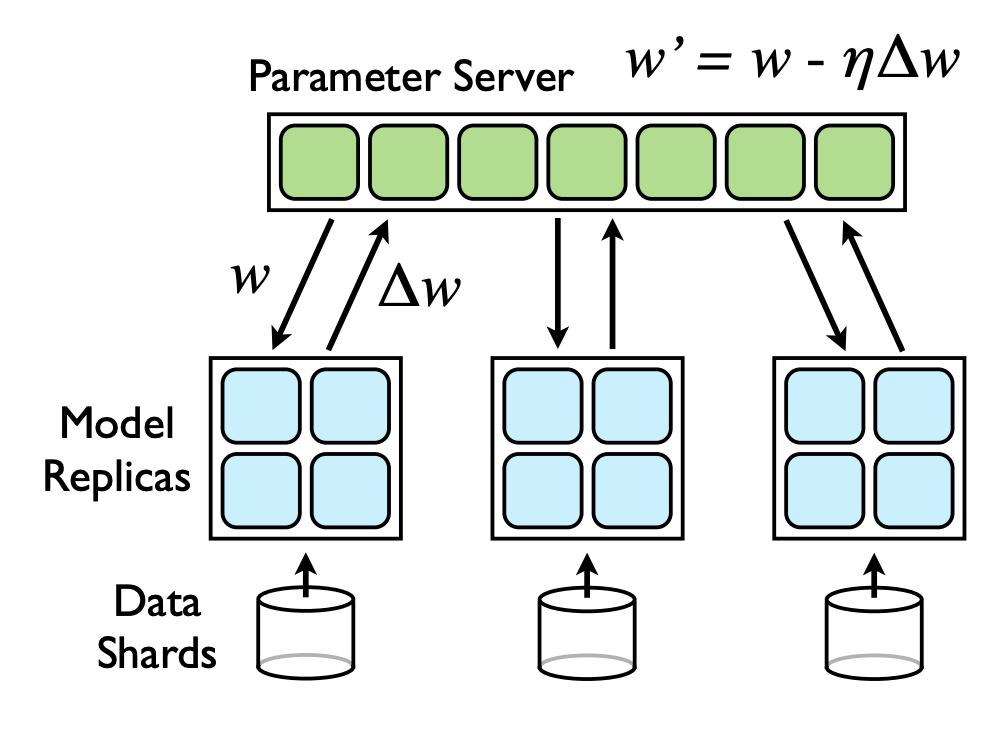
\includegraphics[width=0.7\linewidth]{figures/algos/sgd.png}
    \caption{Async-SGD: Model replicas asynchronously fetch parameters w and push gradients \(\Delta w\) to the parameter server.}
    \label{fig:sgd}
\end{figure}

\clearpage

Since then a couple of different RL algorithms have proposed including:

$\bullet$ \textit{A distributed version of Deep Q-Networks}~\parencite{ong2015distributed} where they adapt the \textit{DistBelief} software framework to the context of efficiently
training reinforcement learning agents to distribute the deep Q-network training. resulting the method is completely asynchronous and scales well with the number of machines. 

$\bullet$ \textit{Massively parallel methods for DRL}~\ref{fig:gorila} \textbf{(Gorilla)}~\parencite{nair2015massively}, which uses a distributed experience replay buffer (and no prioritization). This architecture~\ref{fig:gorila_arch} uses four main components: \textit{parallel actors} that generate new behaviour, \textit{parallel learners} that are trained from stored experience, \textit{a distributed neural network} to represent the value function or behaviour policy, and \textit{a distributed store of experience} with no prioritization. It was applied to \textbf{49 games} from Atari 2600 games from the Arcade Learning Environment, using identical hyperparameters. The performance~\ref{fig:gorila_results} surpassed \textit{non-distributed DQN} in \textbf{41} of the 49 games and also reduced the wall-time required to achieve these results by an order of magnitude on most games.

\begin{figure}[H]
	\centering
	\begin{subfigure}[b]{0.4\textwidth}
		\centering
		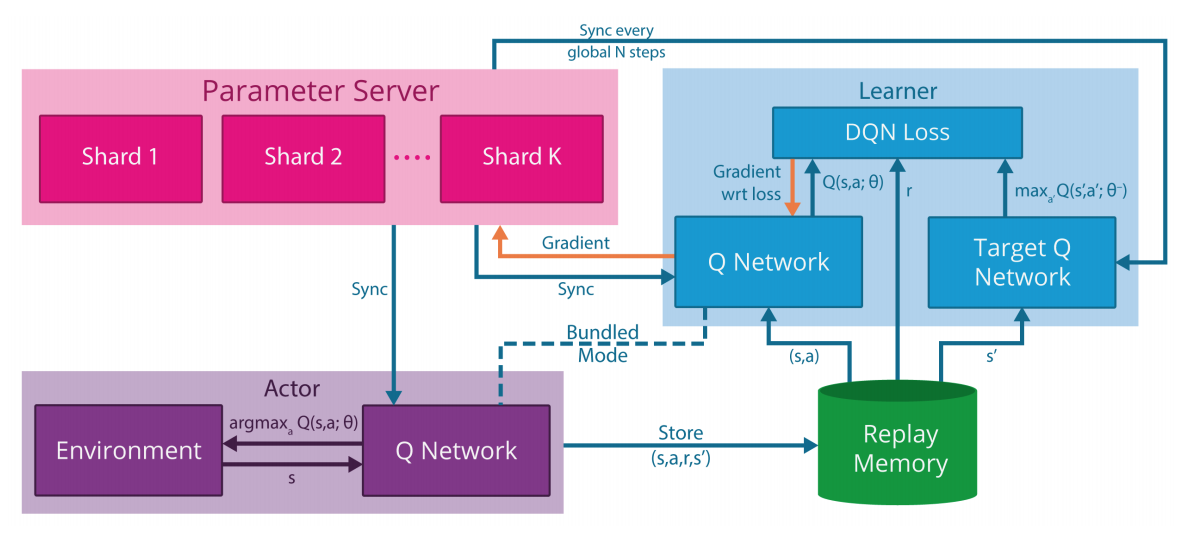
\includegraphics[width=\textwidth]{figures/algos/gorila.png}
		\caption{Agent parallelises the training procedure by separating out learners, actors and parameter server}
		\label{fig:gorila_arch}
    \end{subfigure}
    \hfill
	\begin{subfigure}[b]{0.4\textwidth}
		\centering
		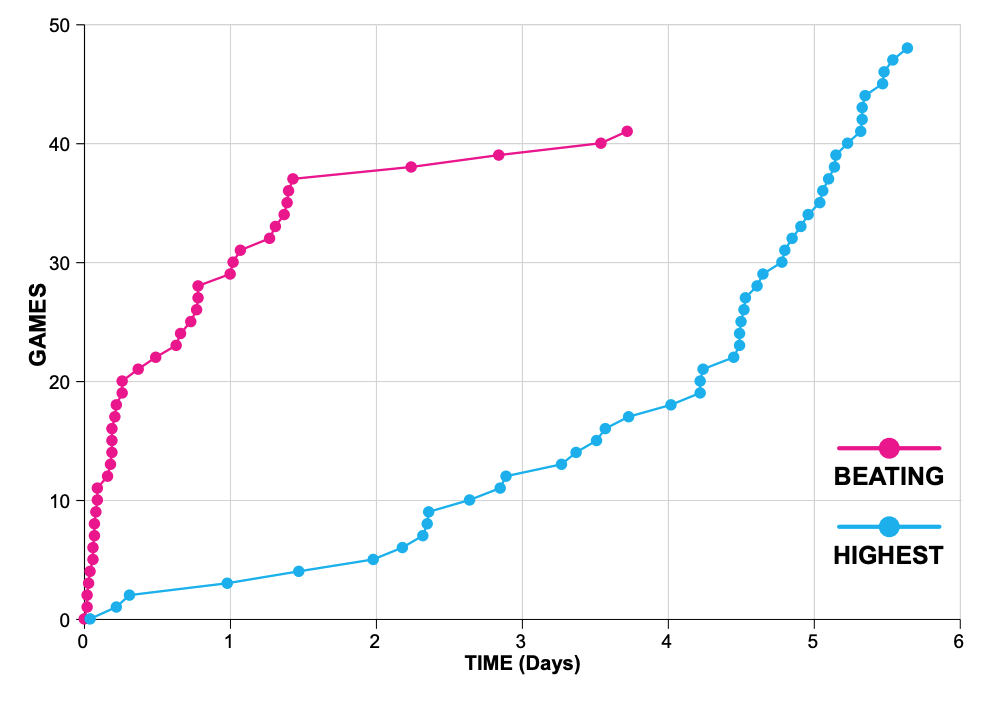
\includegraphics[width=\textwidth]{figures/algos/gorila_results.png}
        \caption{Red curve: time to surpass single DQN\\
                Blue curve: time to reach its peak performance}
		\label{fig:gorila_results}
	\end{subfigure}
	\hfill
	   \caption{The Gorila Architecture \& Results}
	   \label{fig:gorila}
\end{figure}

$\bullet$ \textit{Asynchronous methods for DRL}~\ref{fig:a3c} \textbf{(A3C)}~\parencite{mnih2016asynchronous}, in which they present asynchronous variants of four standard reinforcement learning algorithms and show that parallel actor-learners have a stabilizing effect on training allowing all four methods to successfully train neural network controllers using asynchronous gradient descent for optimization. The algorithms~\ref{fig:a3c_workflow} used multiple threads to run copies of the environment and generate uncorrelated sequences of training samples. Parameters were then sent to a shared parameter server at regular intervals. Because this promotes non-stationarity for the sequences of SARSA tuples, experience replay is not necessarily needed. The implementations of RMSProp and Momentum SGD used by the authors employed a Hogwild-inpsired~\parencite{recht2011hogwild} lock free scheme for maximum efficiency. A3C is the ``best'' agent that was presented in this paper. It is an asynchronous advantage actor-critic algorithm. It maintains an approximation of the policy, an estimate of the value function, and computes an ``advantage'' function and a variance-reducing baseline~\parencite{degris2012off}. An entropy regularization term was also used to discourage premature convergence. The A3C performance overpassed gorila and add some enhancement including faster updates, removing  the replay buffer, and moving to Actor-Critic (from Q learning).

The State-of-the-art results~\ref{fig:a3c_results} were obtained on some of the Atari games (ALE). An LSTM-based A3C agent was tested with Deepmind’s Labyrinth environment. They also tested on the TORCS car racing environment and MuJoCo, the continuous-space physics simulation engine.

\begin{figure}[H]
	\centering
	\begin{subfigure}[b]{0.3\textwidth}
		\centering
		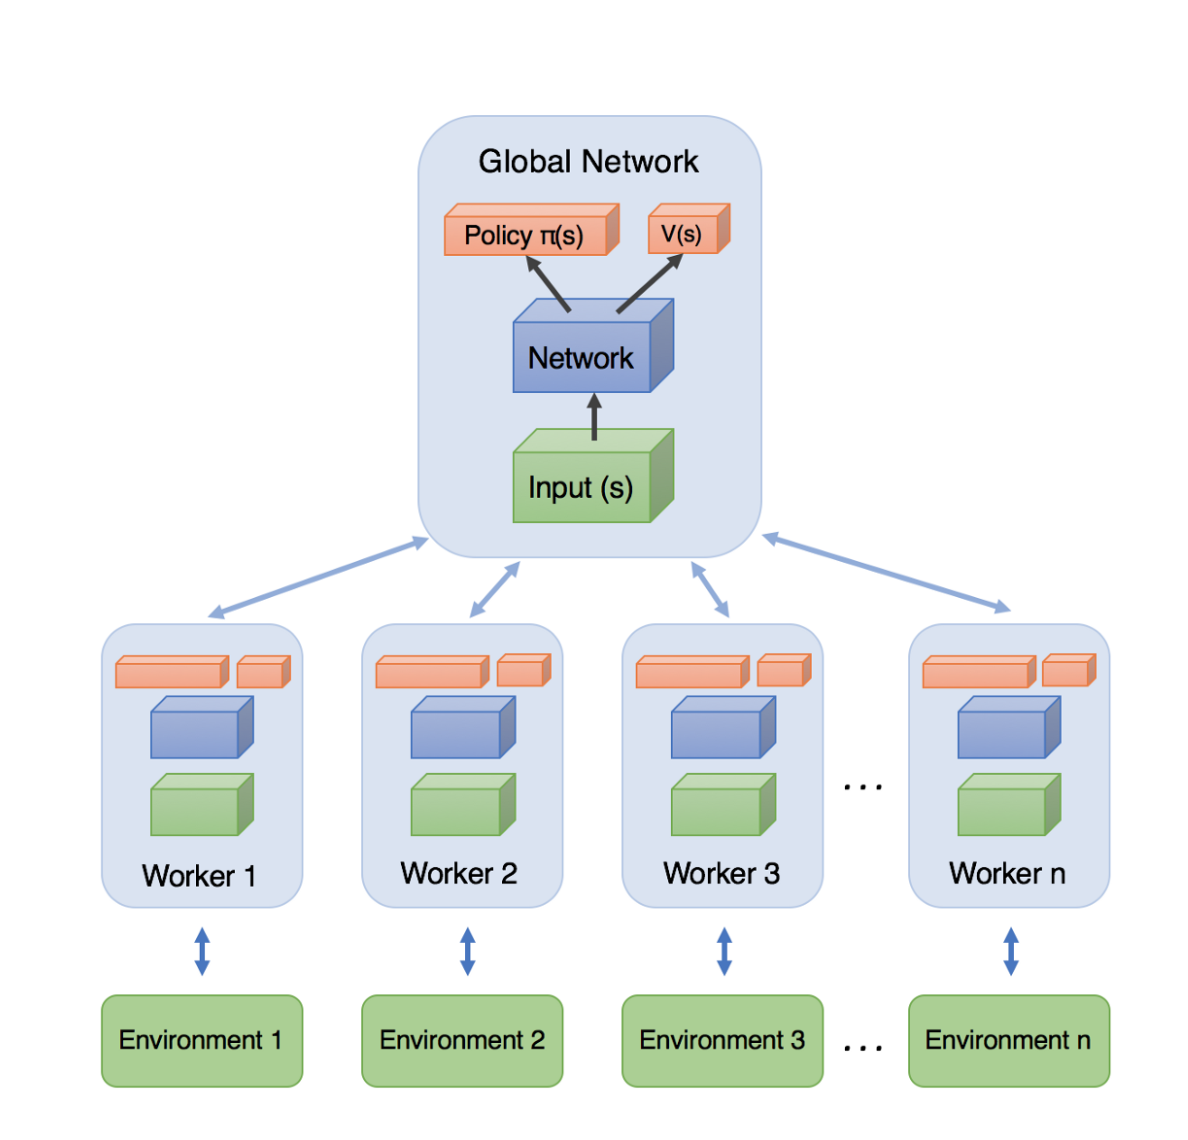
\includegraphics[width=\textwidth]{figures/algos/a3c.png}
		\caption{A3C high-level architecture.}
		\label{fig:a3c_arch}
    \end{subfigure}
    \hfill
    \begin{subfigure}[b]{0.3\textwidth}
		\centering
		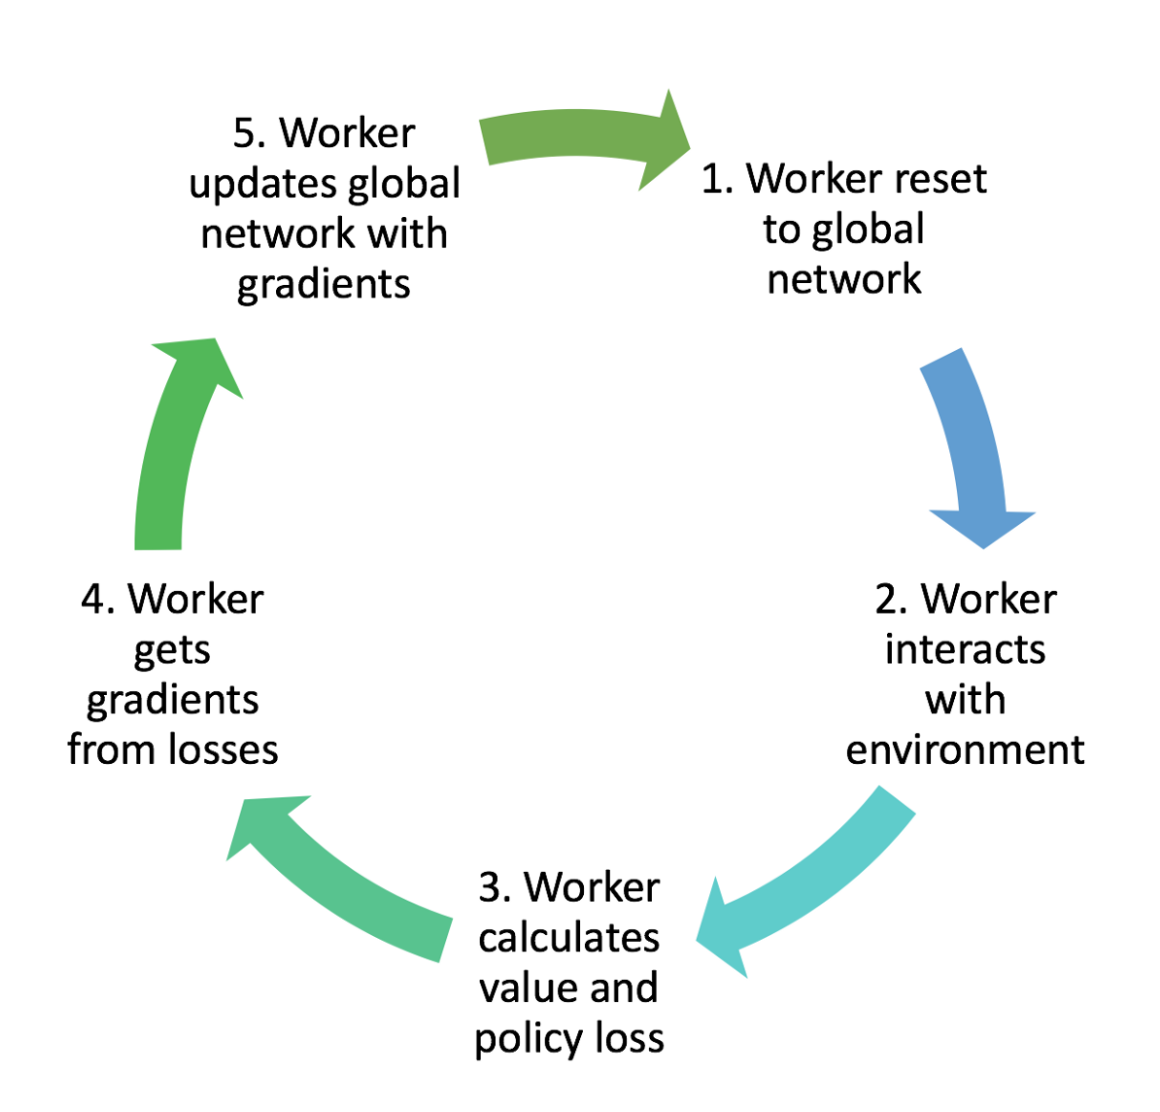
\includegraphics[width=\textwidth]{figures/algos/a3c_workflow.png}
		\caption{Training workflow of each worker agent in A3C.}
		\label{fig:a3c_workflow}
    \end{subfigure}
    \hfill
	\begin{subfigure}[b]{0.3\textwidth}
		\centering
		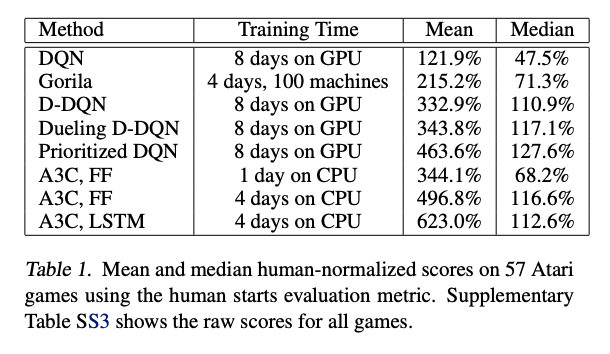
\includegraphics[width=\textwidth]{figures/algos/a3c_results.png}
        \caption{A3C Results}
		\label{fig:a3c_results}
	\end{subfigure}
	\hfill
	   \caption{The A3C Architecture, workflow \& Results}
	   \label{fig:a3c}
\end{figure}

Another direction with some alternatives to \textit{asynchronous SGD} methods which includes distributed BA3C~\parencite{adamski2018distributed}, Evolution strategies~\parencite{salimans2017evolution} using evolutionary processes and 

$\bullet$ \textit{Distributed Prioritized Experience Replay}~\ref{fig:apex} \textbf{(Ape-X)}~\parencite{horgan2018distributed} which use a distributed replay with a synchronous learner. They focused on on applying the Ape-X framework to DQN and DPG, also it could  be combined with any other off-policy reinforcement learning update. 

The main idea of this paper is to scale up the experience replay data by having many actors running in parallel  collect samples of experience. The actors periodically pool their samples into a centralized data repository, which is used for experience replay for a centralized learner to select from it in a prioritized fashion~\parencite{schaul2015prioritized} and update neural network parameters. Those parameters then get copied back to the actors. Hence, they step over and complement standard distributed training approaches~\parencite{dean2012large} of neural networks which focus on parallelizing the computation of gradients to \textit{distribute the generation and selection of experience data}, which suffices to improve results.

This architecture achieved state of the art results~\ref{fig:apex_results} in a wide range of discrete and continuous tasks, both in terms of wall-clock learning speed and final performance

\begin{figure}[H]
	\centering
	\begin{subfigure}[b]{0.4\textwidth}
		\centering
		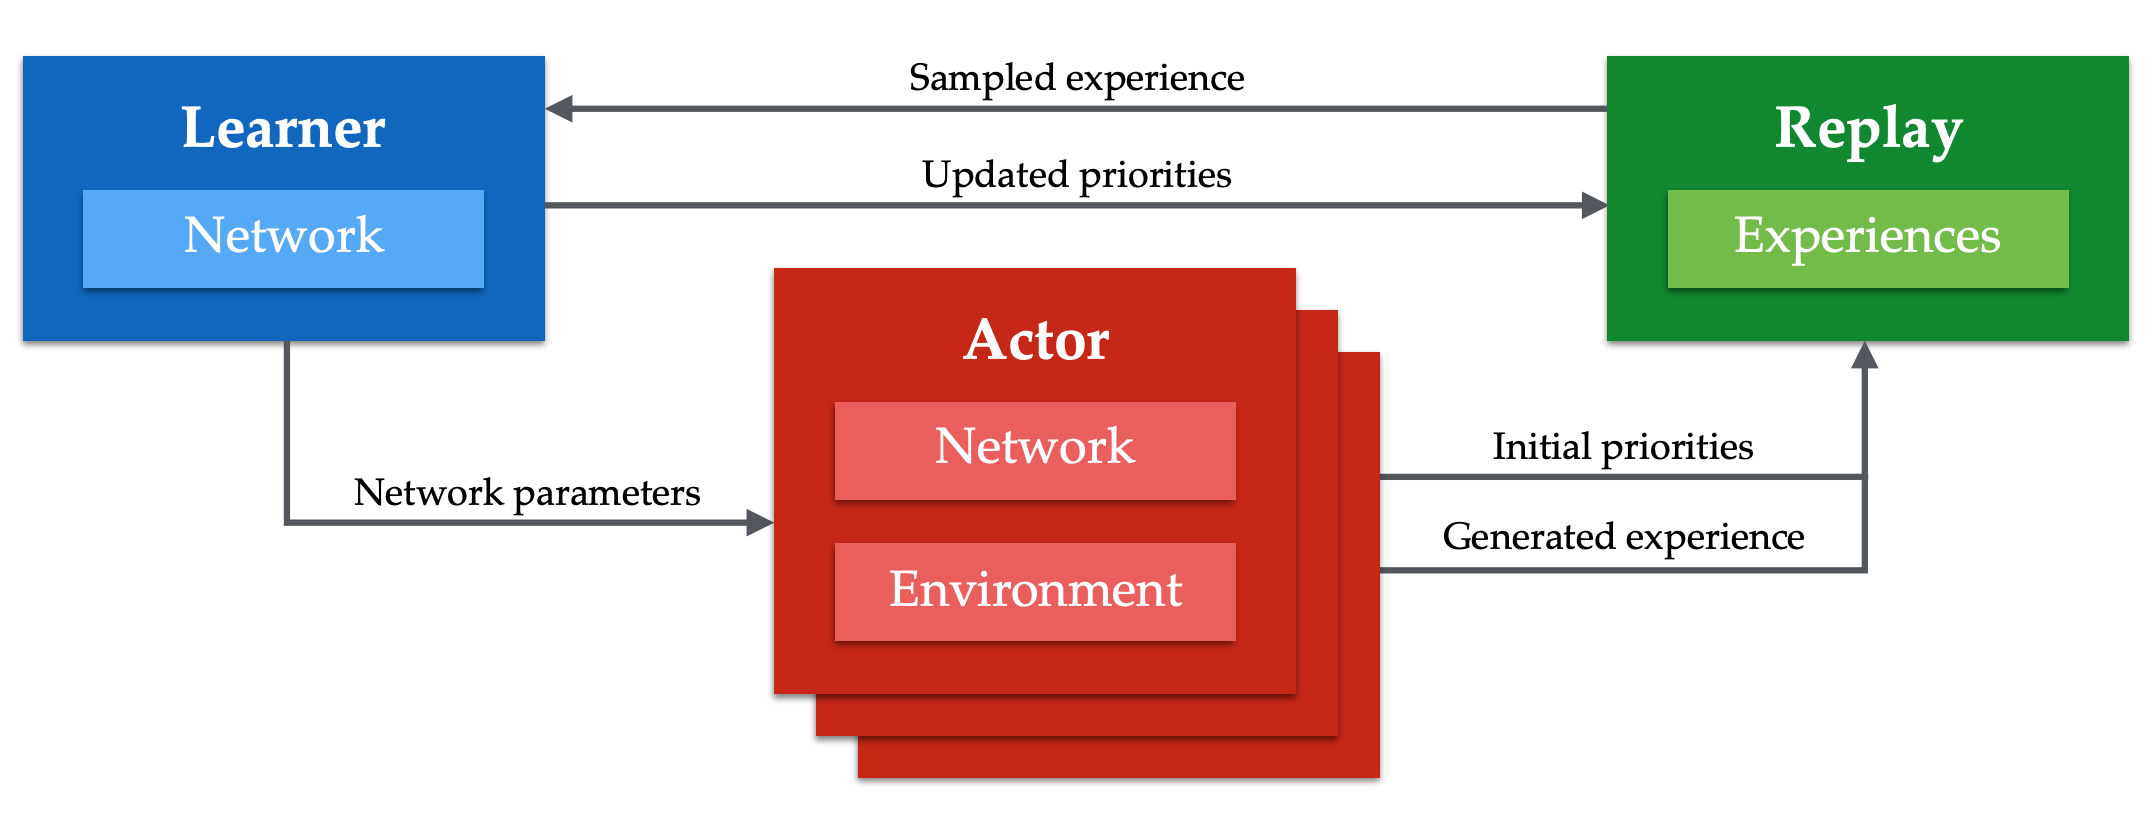
\includegraphics[width=\textwidth]{figures/algos/apex.png}
		\caption{The Ape-X architecture}
		\label{fig:apex_arch}
    \end{subfigure}
    \hfill
	\begin{subfigure}[b]{0.4\textwidth}
		\centering
		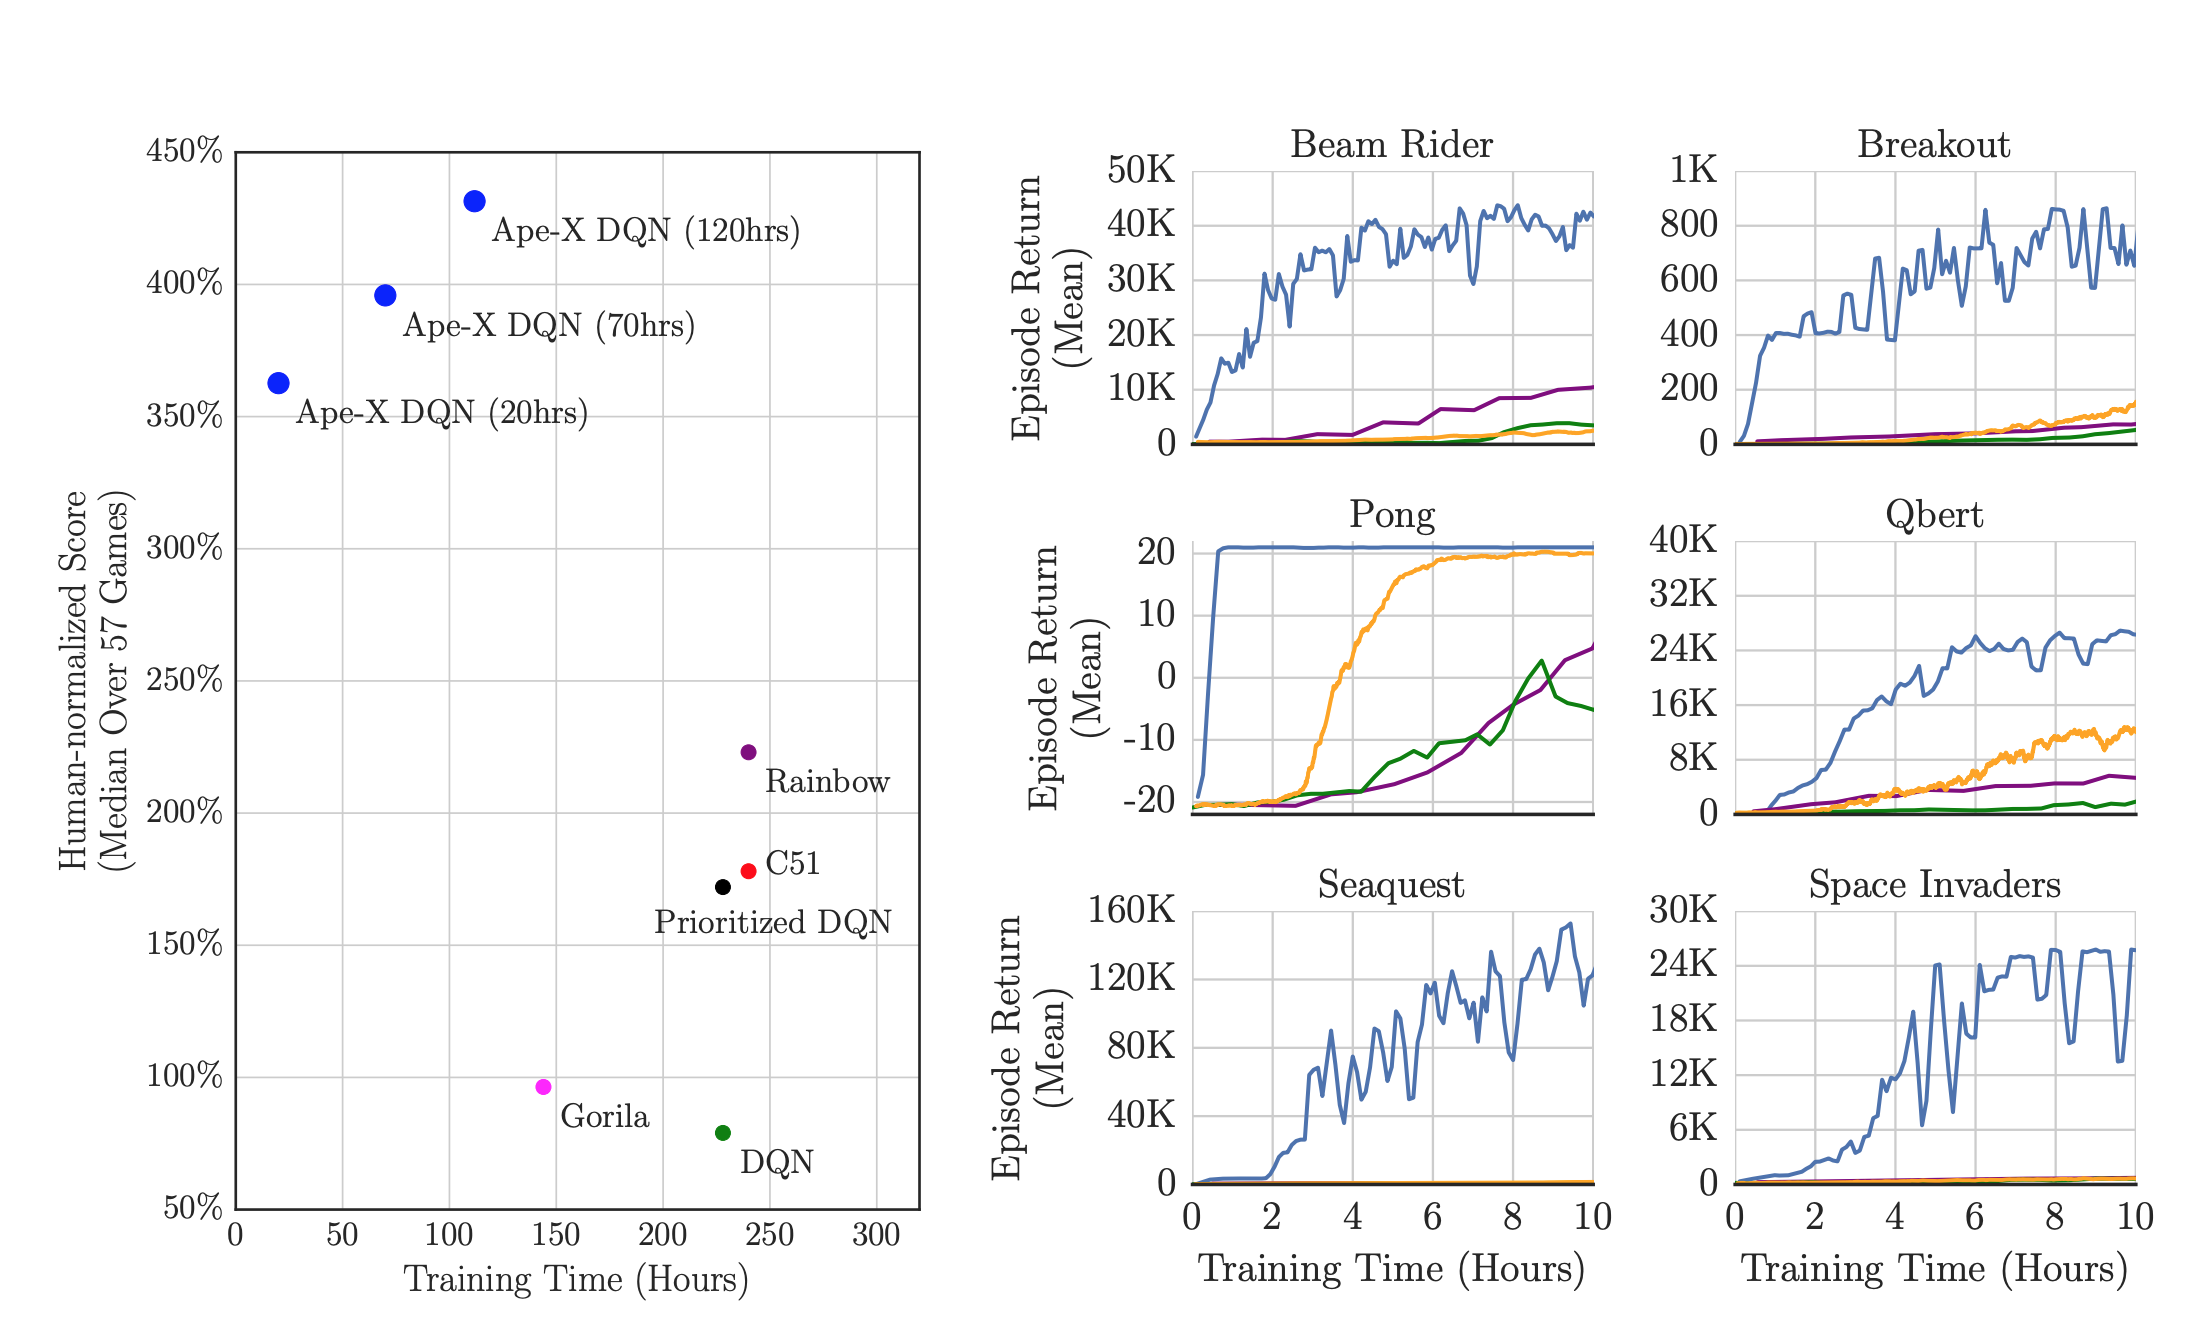
\includegraphics[width=\textwidth]{figures/algos/apex_results.png}
        \caption{Ape-X Performance compared with other RL algorithms}
		\label{fig:apex_results}
	\end{subfigure}
	\hfill
	   \caption{The Ape-X Architecture \& Results}
	   \label{fig:apex}
\end{figure}

Other research have attempt to scale up by using multiple GPUs and utilizing them. The simplest method is batched A2C~\parencite{clemente2017efficient} in which with every step produces a batch of actions and applies them to a batch of environments. BA3C~\parencite{babaeizadeh2016ga3c} another method which uses asynchronous data collection to effectively utilize GPUs.

The most recent work done in the are of distributed deep reinforcement learning and multi-tasking learning which achieve the state of the art performance is \textit{Importance Weighted Actor-Learner Architectures}~\ref{fig:impala} \textbf{(IMPALA)}~\parencite{espeholt2018impala} by DeepMind. It is a scalable distributed DeepRL for their newly designed DMLab-30 environment (which is a collection of new levels designed using our open source RL environment \textit{DeepMind Lab}, These environments are provides to test systems on a large spectrum of interesting tasks either individually or in a multi-task setting).

Importance Weighted Actor-Learner Architecture~\ref{fig:impala_arch} is inspired by the popular \textbf{A3C} architecture which uses multiple distributed actors to learn the agent’s parameters. The developed new distributed agent impala maximizes data throughput using an efficient distributed architecture with TensorFlow. 
In training process for actor-critic methods, each of the actors uses a clone of the policy parameters to act in the environment. Periodically, actors pause their exploration to share the gradients they have computed with a central parameter server that applies updates. 

On the other hand, impala's actors are not used to calculate gradients. Instead, they are just used to \textit{collect experience} which is passed to a \textit{\textbf{central learner}} that computes gradients, resulting in a model that has completely independent actors and learners. 
Separating the learning and acting in this way also has the advantage of increasing the throughput of the whole system since the actors no longer need to wait for the learning step like in architectures such as batched A2C~\ref{fig:impala_vs_a2c}. This allows us to train impala architectures on interesting environments without suffering from variance in frame rendering-time or time consuming task restarts.

However, decoupling the acting and learning causes the policy in the actor to lag behind the learner. In order to compensate for this difference we introduce a principled off-policy advantage actor critic formulation called V-trace which compensates for the trajectories obtained by actors being off policy.

Importance Weighted Actor-Learner Architecture was 10 times more data efficient and achieved double the final score compared to distributed A3C~\ref{fig:impala_results}.  Moreover, Importance Weighted Actor-Learner Architectures showed positive transfer from training in multi-task settings compared to training in single-task setting.

\begin{figure}[H]
	\centering
	\begin{subfigure}[b]{0.3\textwidth}
		\centering
		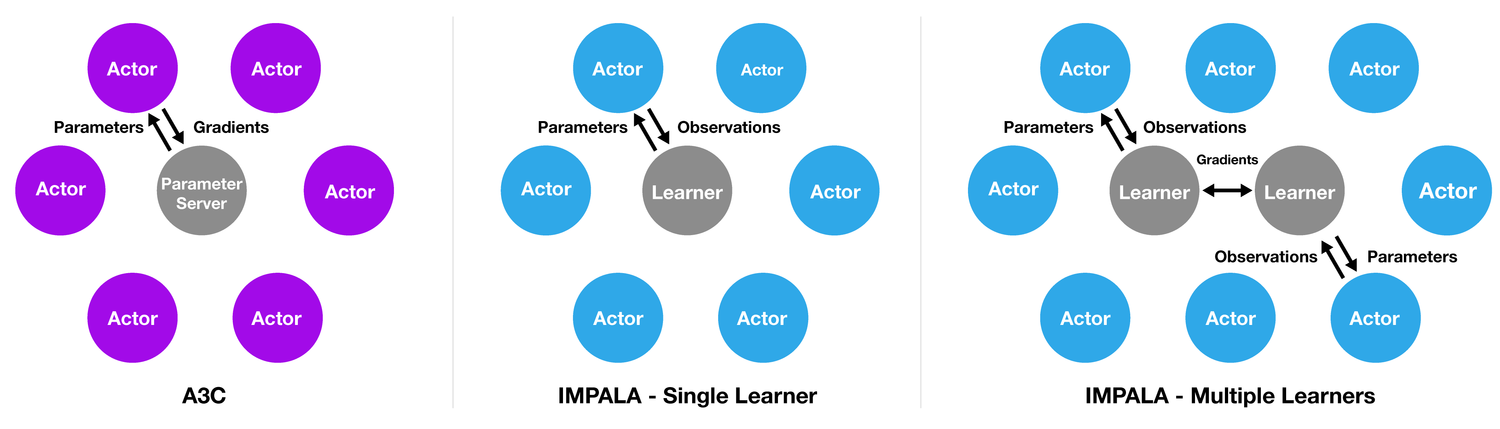
\includegraphics[width=\textwidth]{figures/algos/impala.png}
		\caption{The IMPALA Architecture.}
		\label{fig:impala_arch}
    \end{subfigure}
    \hfill
    \begin{subfigure}[b]{0.3\textwidth}
		\centering
		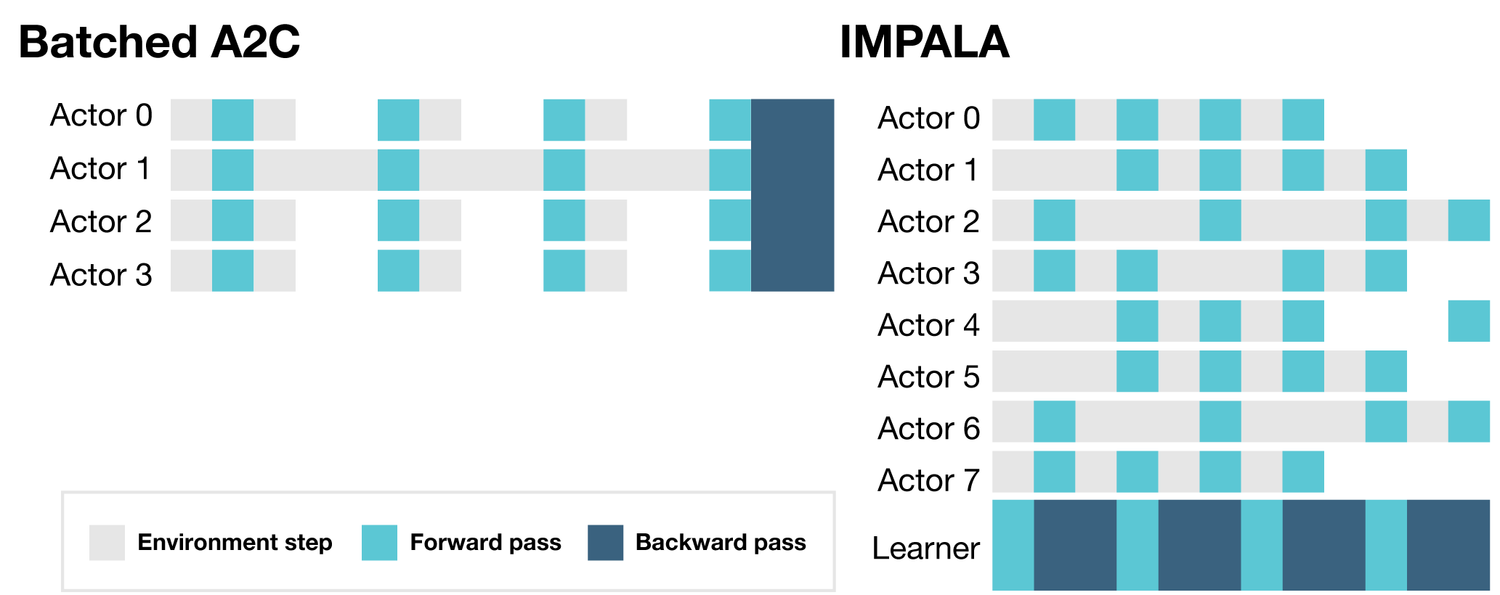
\includegraphics[width=\textwidth]{figures/algos/impala_vs_a2c.png}
		\caption{IMPALA vs Batched A2C Training}
		\label{fig:impala_vs_a2c}
    \end{subfigure}
    \hfill
	\begin{subfigure}[b]{0.3\textwidth}
		\centering
		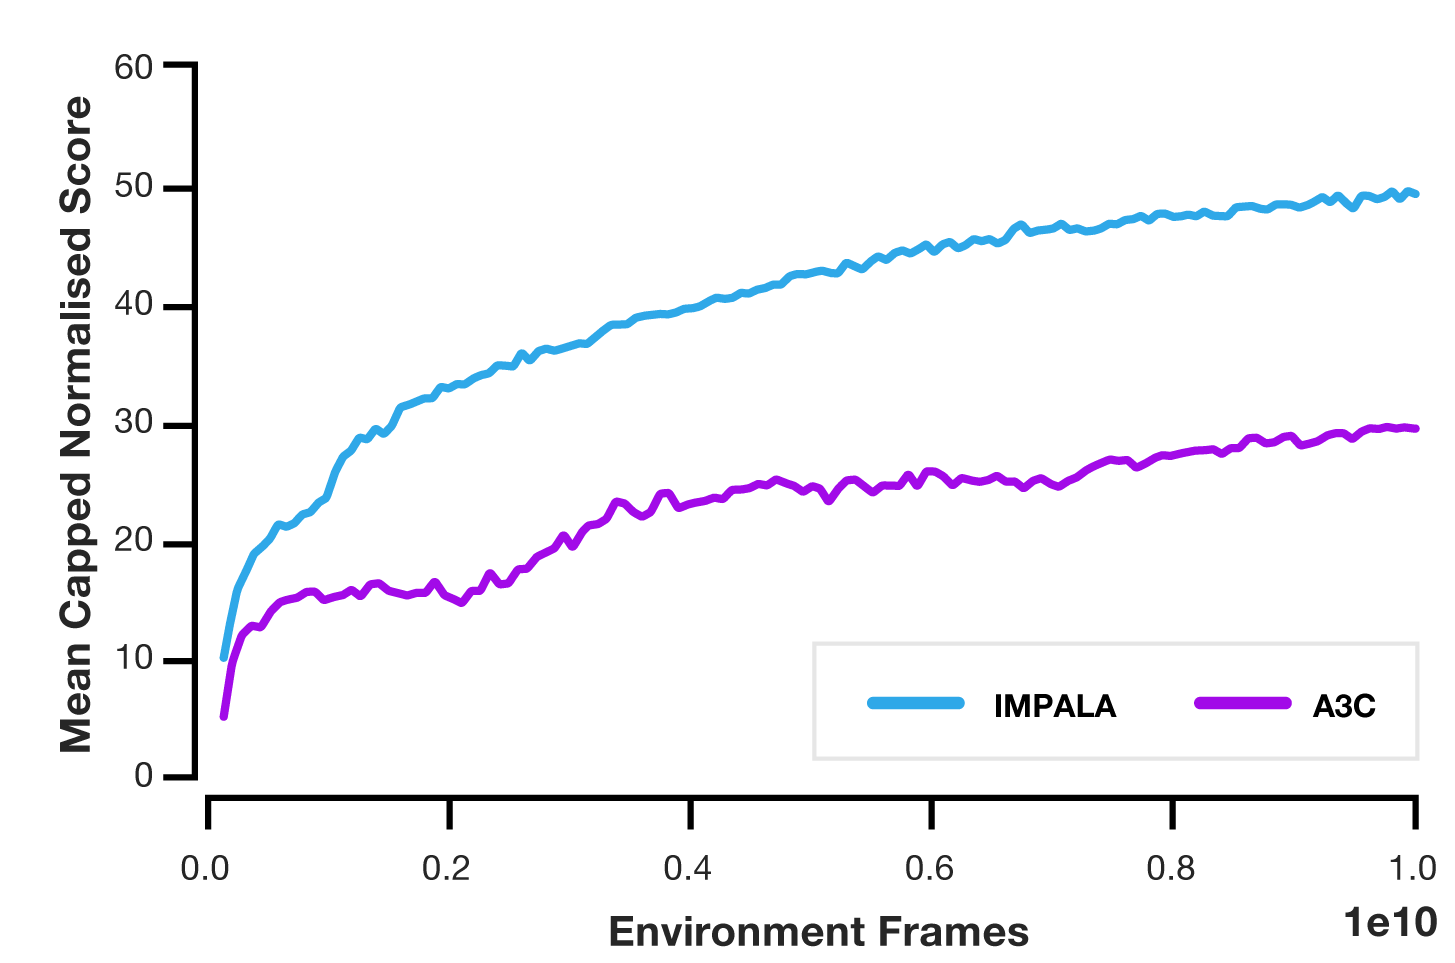
\includegraphics[width=\textwidth]{figures/algos/impala_results.png}
        \caption{IMPALA Results}
		\label{fig:impala_results}
	\end{subfigure}
	\hfill
	   \caption{The IMPALA Architecture, Comparison \& Results}
	   \label{fig:impala}
\end{figure}

On the practical side, there have been some frameworks developments that focuses on distributed deep reinforcement learning and applying all the techniques and algorithms to multiple environments for the sake of advancing DRL research. Dopamine~\parencite{castro2018dopamine} is a new framework for flexible and reproducible Reinforcement Learning Research by google in which they provide large-scale distributed training and enabling distributing the learning process across multiple workers, with distributional methods that allow agents to model full distributions, rather than simply their expected values, to learn a more complete picture of their world. This framework aims to provide flexibility, stability, and reproducibility for new and experienced RL researchers alike. Inspired by one of the main components in \textit{reward-motivated behaviour (dopamine)} in the brain and reflecting the strong historical connection between neuroscience and reinforcement learning research.

Ray~\parencite{moritz2018ray} is another more general framework with Distributed Execution for AI Applications. Ray is a high-performance distributed execution framework targeted at large-scale machine learning and reinforcement learning applications. It achieves scalability and fault tolerance by abstracting the control state of the system in a global control store and keeping all other components stateless. It uses a shared-memory distributed object store to efficiently handle large data through shared memory, and it uses a bottom-up hierarchical scheduling architecture to achieve low-latency and high-throughput scheduling. It uses a lightweight API based on dynamic task graphs and actors to express a wide range of applications in a flexible manner.


\section{Research Statement}
In this research project, our aim is to apply a set of reinforcement learning algorithms (distributed and non-distributed architectures) to multiple different existing environments and run some experiments in normal non-distributed setup and parallel and distributed setup to measure the effect of the training modes and compare the performance among these environments and see the effect of the distribution. 

We will be comparing between the state of the art algorithms mentions above in the related work and we will be using Ray framework as our backend for the experiments along with some of the implemented algorithms. 

We created will create abstract class to unify the different RL environments to provide clarity and simplicity to deal with the environments and to be easy to use with other existing frameworks.

In our work, we will be demonstrating full benchmarking for all the experiments we have done along with comparisons between all of the environments and applied algorithms.

\section{Overview and Outline}
The work is organized as follows. In \autoref{chapter:Background and Foundations}, the theoretical background linked to reinforcement learning and the Markov decision process framework are introduced. Furthermore, we discuss the use of deep learning in RL framework and the state of the art algorithms, we also discuss the challenging problems associated with reinforcement learning.  The \autoref{chapter:Background and Foundations} presents the experiment setting used in \autoref{chapter:Background and Foundations}. The latter presents, examines and discusses the results. Finally, \autoref{chapter:Background and Foundations} discusses future work and concludes.